\chapter{Problem introduction}
Through this project we intend to become familiar with imbalanced multi-class supervised classification problems. To serve this purpose, we decided to explore the Forest Cover type dataset in the UCI Machine Learning Repository. The dataset comprises observations taken from 30m by 30m patches of the Roosevelt National Forest (in northern Colorado) that are labelled upon the main cover type of that patch.

\section{Dataset overview}
The training set counts $15\,120$ observations while the test set $565\,892$. The data comes from the US Geological Survey
(USGS) and the US Forest Service (USFS) and, in particular, for each patch the following 12 variables (with their units of measure) plus the labels are provided:
\begin{enumerate}
	\item Elevation (m),
	\item Aspect (azimuth from true north),
	\item Slope ($^{\circ}$),
	\item Horizontal distance to nearest surface water feature (m),
	\item Vertical distance to nearest surface water feature (m),
	\item Horizontal distance to nearest roadway (m),
	\item Hillshade 9am: a relative measure of incident sunlight at 09:00 h on the summer solstice (index),
	\item Hillshade Noon: a relative measure of incident sunlight at noon on the summer solstice (index),
	\item Hillshade 3pm: a relative measure of incident sunlight at 15:00 h on the summer solstice (index),
	\item Horizontal distance to nearest historic wildfire ignition point (m),
	\item Wilderness area: the macro-area the patch belongs to (four binary values, one for each wilderness area),
	\item Soil type: the principal soil type in the patch (40 binary values, one for each soil type),
	\item Cover type: forest cover type (classes from 1 to 7, one for each patch).
\end{enumerate}
Table \ref{tab:covertypes} shows that the dataset is imbalanced. Requiring a training set where all classes are equally represented, it is necessary to reduce the size of the former. Therefore, according to \cite{blackardDean} the training set (which includes the validation data) should follow the approach of Figure \ref{fig:covertypesdims}. The relative sizes of the train and test sets make the classification a challenging problem, because the train set is $\sim2.6\%$ of the overall dataset.
\begin{table}[]
	\centering
	\begin{tabular}{ll}
		Cover type & Occurrences \\
		1          & $211\,840$  \\
		2          & $283\,301$  \\
		3          & $35\,754$   \\
		4          & $2\,747$    \\
		5          & $9\,493$    \\
		6          & $17\,367$   \\
		7          & $20\,510$   \\
		Total      & $581\,012$     
	\end{tabular}
	\caption{Number of observations within each forest cover type class}
	\label{tab:covertypes}
\end{table}
\begin{figure}
	\centering
	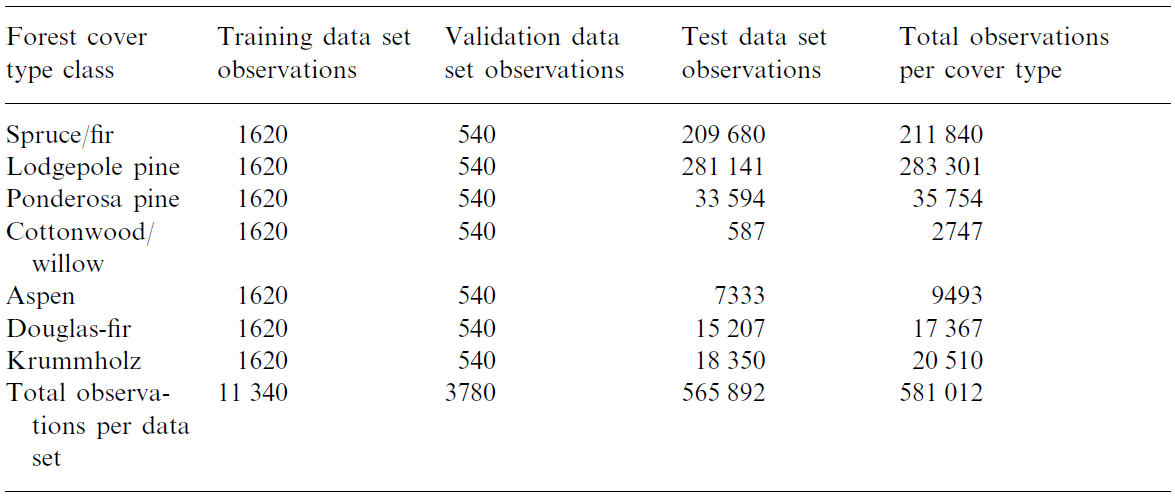
\includegraphics[width=\textwidth]{./TeX_files/img/covertypetable.png}
	\caption{Number of observations within each forest cover type class for each data set}
	\label{fig:covertypesdims}
\end{figure}

\section{Feature engineering}
The total amount of features is 54, thus, a simple manual feature selection is applied. It is important to notice that the analysis, from now on, has been done on the training set only (to avoid data contamination). For example, Figure \ref{fig:elevationhist} shows the elevation grouped by each cover type; it is quite clear that classes 4 (Cottonwood/Willow), 5 (Aspen) and 7 (Krummholz) are separable. Focusing on the numerical features, Figure \ref{fig:fullcorrmatrix} shows the correlation plots for each of them. Therefore, the most interesting positive correlation results are $0.6521$ and $0.6145$ for the couples <<Vertical\_Distance\_To\_Hydrology - Horizontal\_Distance\_To\_Hydrology>> and <<Hillshade\_Noon - Hillshade\_3pm>>, respectively. While for the negative correlation there is $-0.7800$ for the couple <<Hillshade\_9am - Hillshade\_3pm>>. From these observations, two new features could substitute the ones used for their computation allowing us to reduce the feature space:
\begin{itemize}
\item Distance\_To\_Hydrology: the Euclidean distance computed on Vertical\_Distance\_To\_Hydrology and Horizontal\_Distance\_To\_Hydrology,
\item Mean\_Hillshade: the mean value of the three Hillshade features.
\end{itemize}
Moreover Hillshade\_3pm missing values ($88$ zeros) have been imputed with the median over all the training samples and one-hot encoding has been applied to the target variable yielding 7 binary variables. Finally, all the numerical features were scaled with zero mean and unit variance.
\begin{figure}
\centering
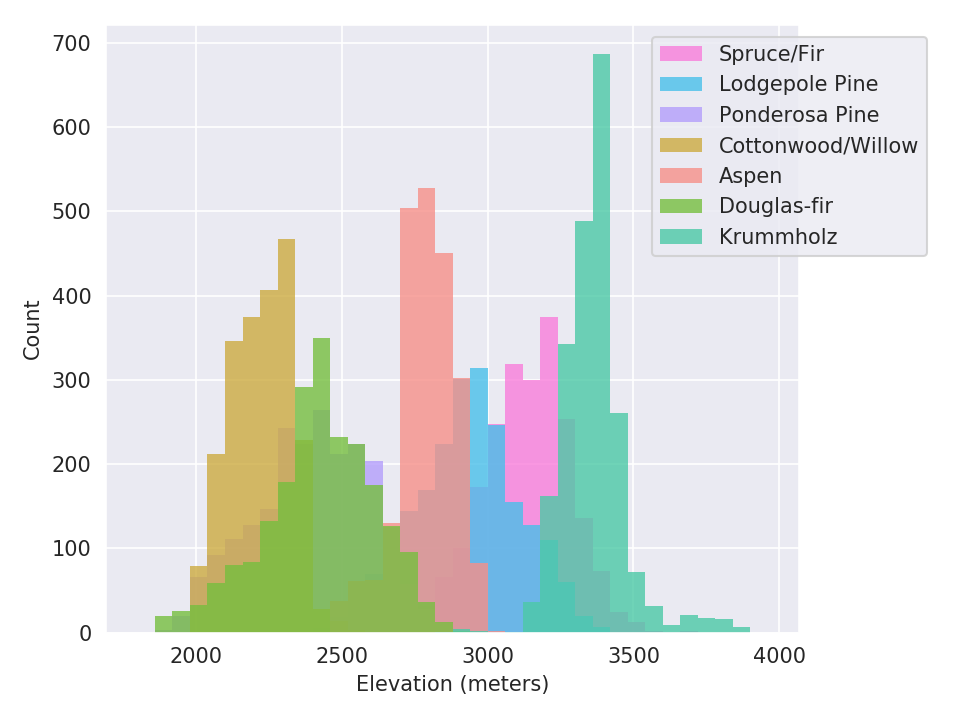
\includegraphics[width=\textwidth]{./TeX_files/img/elevationhist.png}
\caption{Elevation histogram for each cover type. At a first glance classes 4 (Cottonwood/Willow), 5 (Aspen) and 7 (Krummholz) are easily separable.}
\label{fig:elevationhist}
\end{figure}
\begin{sidewaysfigure}
\centering
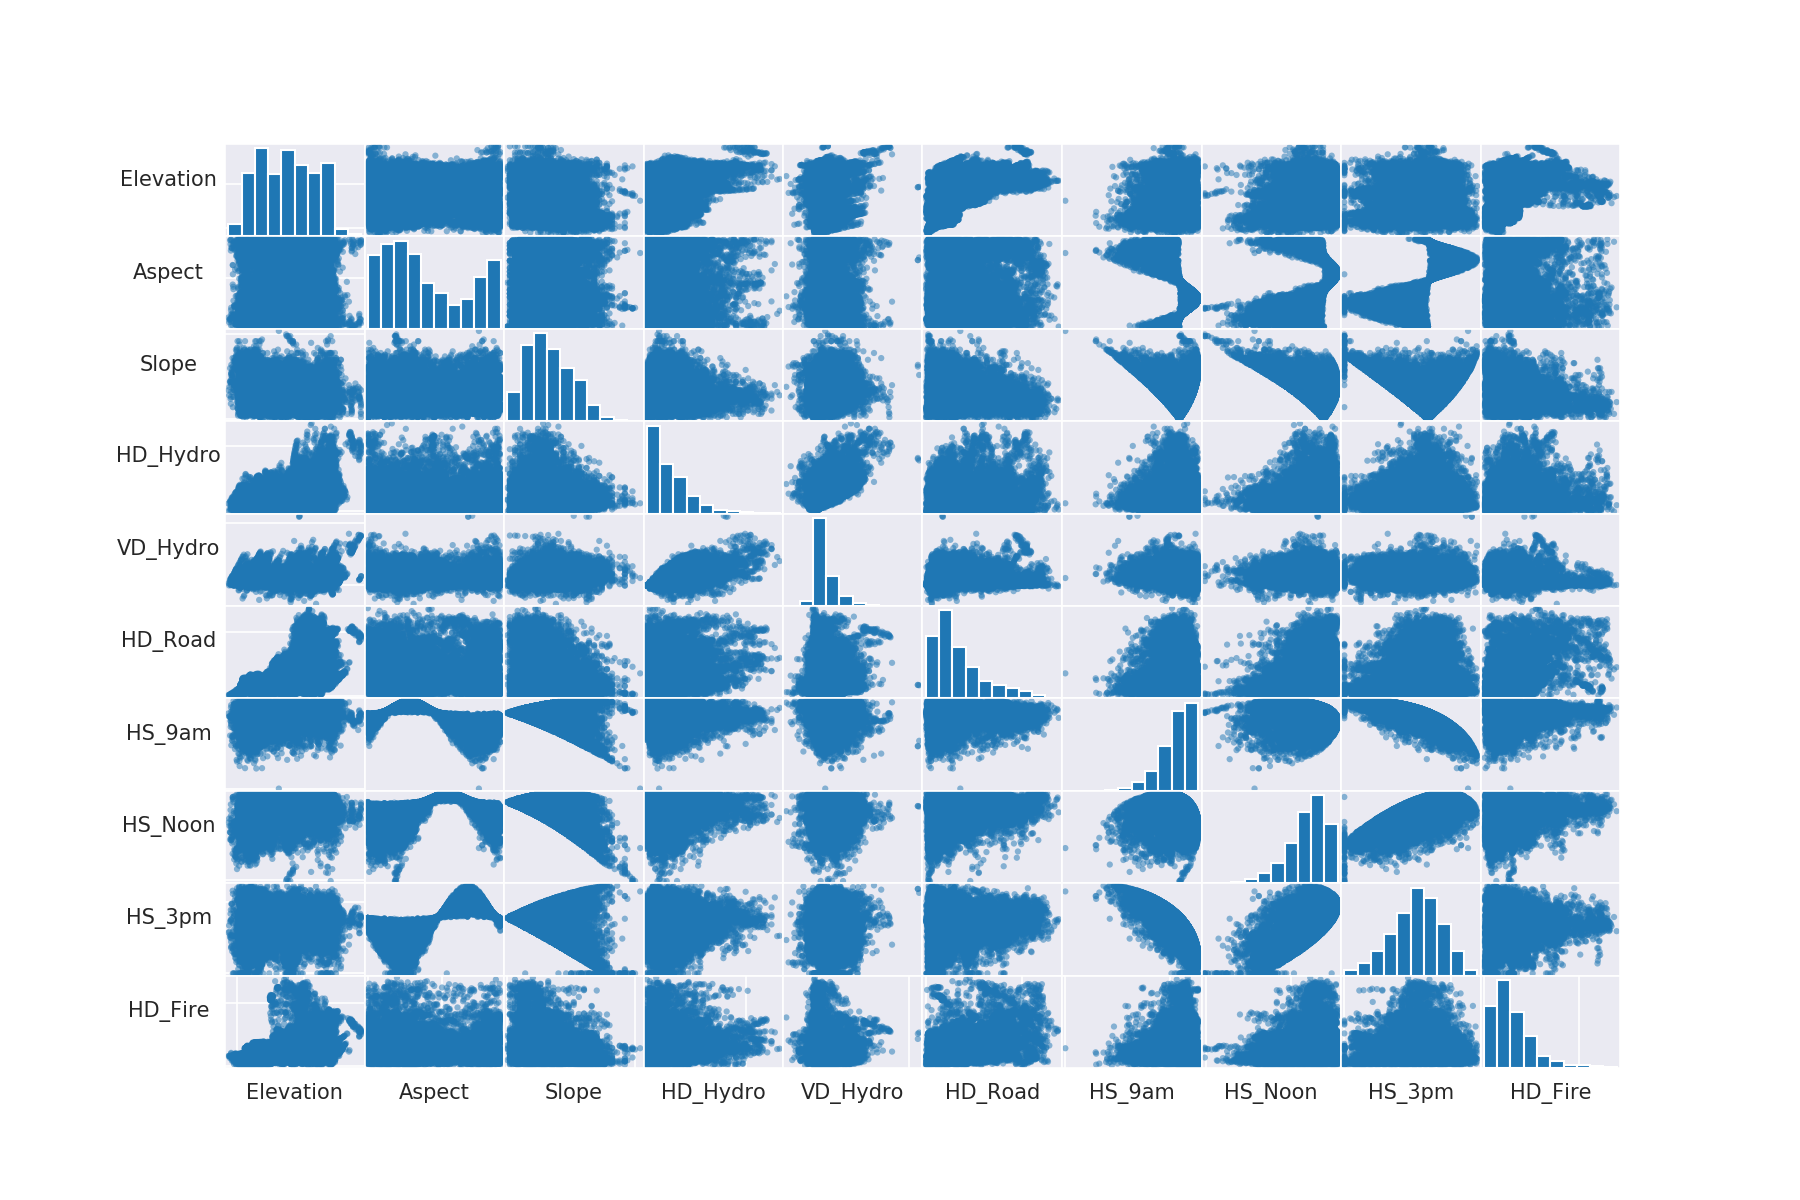
\includegraphics[width=\textwidth]{./TeX_files/img/fullcorrmatrix.png}
\caption{Correlation matrix of the numerical features.}
\label{fig:fullcorrmatrix}
\end{sidewaysfigure}